\section{Raspberry pi}
Raspberry Pi is a small computer, with everything gathered in one board. In our project we will be using the B model, revision 2, which have a 700MHz ARM CPU, 512MB of RAM and a SC-card reader, in addition to the leads to connect to different devices, for  the full overview, see figure \ref{fig:raspberrypihighlevel}. The recommended operating system is Raspbian, a linux distribution based on Debian. 

The Raspberry pi was originally intended to help teach programming, but it can also perform many of the standard computer tasks, and it can be connected to a monitor or tv using an HDMI lead. In our project we hope to be able to use a Raspberry pi to run the software required to control the ground stations. The software provided by the Carpcomm project has Raspbian as one of its supported platforms, so we hope this will work well.

\begin{figure}
	\begin{center}
		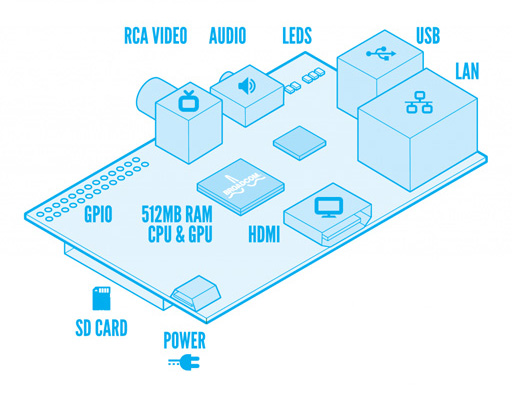
\includegraphics[width=0.7\textwidth]{Figures/raspberrypi_modelb_hl.jpg}
	\end{center}
	\caption[Raspberry pi highlevel]{A highlevel schemantic of the Raspberry pi, model B rev 2}
	\label{fig:raspberrypihighlevel}
\end{figure}

To control the movement of the antennas, an serial port is needed. Raspberry Pi has an serial port included in its gpio (general purpose input/output) connector. This serial port uses ttl-standard for its voltage levels, this is 0/3.3V while RS232 which is the standard used in computers uses (3V-15V)/-(3V-15V). Because of this an converter is needed. We chose to make an custom circuit board using the MAX3232 RS232 line driver. The circuit board is designed to be mounted on the gpio connector, because of small space in the case for the Raspberry Pi, the output is connected with cable to the external connector.

\begin{figure}
	\begin{center}
		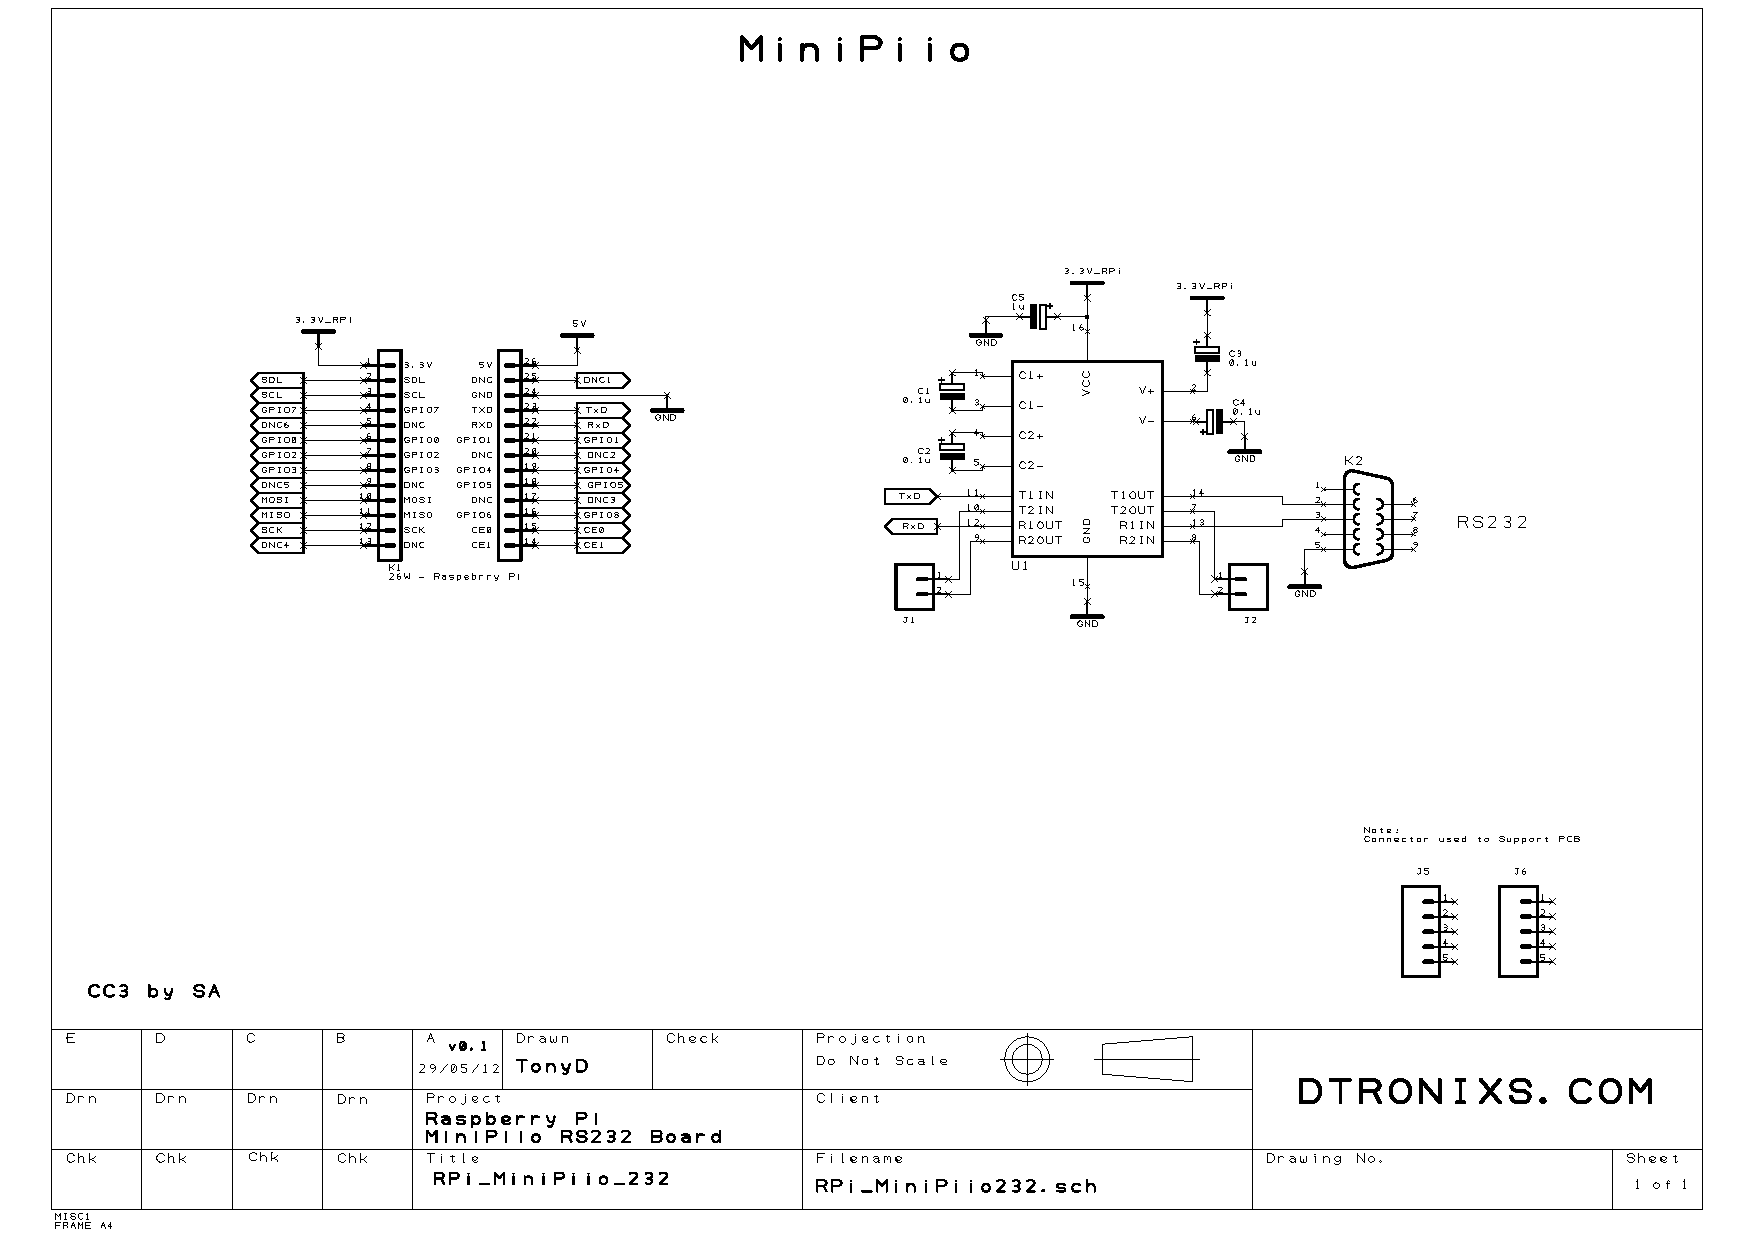
\includegraphics[width=0.7\textwidth, trim=400 250 100 100, clip=true]{../Schematics/UART-to-RS232.pdf}
	\end{center}
	\caption{Schematics for the RS232-converter}
	\label{fig:UART-RS232}
\end{figure}